\chapter{Work Plan}%
\label{chapter:workPlan}

\begin{introduction}
In this chapter, i will explain the work plan for the development of the applications and the writing of the dissertation.
\end{introduction} 


\section{Work Plan}

In the next few month i will develop the first version of the applications according to the use cases i defined in the chapter III. 
I will devide the development in 6 two week long sprints, with two contingicy week, one between the sprint 3 and 4 and another after sprint 6 in case of delay of some tasks.

The Sprint 1 will be dedicated to the integration with the System LightMobie System and the development of the Receptionist Use Cases.  

\begin{itemize}
  \item Integration with the Sytem;
  \begin{itemize}
      \item Start Date: 24/01/2025 
      \item End Date: 27/01/2025 
  \end{itemize}
    \item Receptionist use Cases;
    \begin{itemize}
        \item Start Date: 28/01/2025 
        \item End Date: 06/02/2025 
    \end{itemize}
  \end{itemize}

In the Sprint 2, I will be develop the first five Use Cases of the Mecanic.  

\begin{itemize}
  \item Mecanic Use cases 2.1 - 2.5;
    \begin{itemize}
      \item Start Date: 07/02/2025 
      \item End Date: 20/02/2025 
  \end{itemize}
\end{itemize}

In the Sprint 3, I will develop the last two Use Cases of the Mecanic.  

  \begin{itemize}
    \item Mecanic Use Cases 2.6 and 2.7;
    \begin{itemize}
      \item Start Date: 21/02/2025 
      \item End Date: 06/03/2025 
  \end{itemize}
\end{itemize}

The following week is reserved for the contingicy, so in the case of no delay i can move on to the next sprint, Sprint 4.
In the Sprint 4, I will develop the Admin Use Cases from 4.3 to 4.5. I will skip the 4.1 and 4.2 since they are related to the Warehouse Use Cases.

    \begin{itemize}
      \item Admin Use Cases 4.3 - 4.5;
    \begin{itemize}
      \item Start Date: 14/03/2025 
      \item End Date: 27/03/2025 
  \end{itemize}
\end{itemize}

In the Sprint 5, I will develop remaining two Admin Use Cases, and the Warehouse Use Cases.

\begin{itemize}
  \item Admin Use Cases 4.1 and 4.2;
  \begin{itemize}
    \item Start Date: 28/03/2025 
    \item End Date: 06/04/2025 
  \end{itemize}
  \item Warehouse Use Cases;
  \begin{itemize}
    \item Start Date: 07/04/2025 
    \item End Date: 10/04/2025 
  \end{itemize}
\end{itemize}

In the Sprint 6, I will develop the client application Use Cases.

\begin{itemize}
  \item Client App Use Case;
  \begin{itemize}
    \item Start Date: 11/04/2025  
    \item End Date: 24/05/2025 
  \end{itemize} 
\end{itemize}
The following week is reserved for another contingicy.

  Following de development of the applications, i will reserve a week to conduct a user testing with preferelly users related to the subject.
  The next week i will use to apply the notes and suggestion of the experiment provided to the applications and do some code improvements and testing.
  The remaining time will use to finish writing the dissertation, primarly the results and conclusion.
  The literature will accompany all of this proccess, since it may appear another paper or study that my be relevant to my work.
  This information is illustrated in figure \ref{fig:figure1}.

    \begin{figure}[h]
      \caption{Planned Work described as a Gantt Chart. The master thesis is estimated to be at 25\%, the literature progress to be 80\%, the application Use cases at 85\% and the admin Use Cases at 10\%. The admin Use Cases are at 10\% since they is apart already developed in the LightMobie System.}
      \centering
      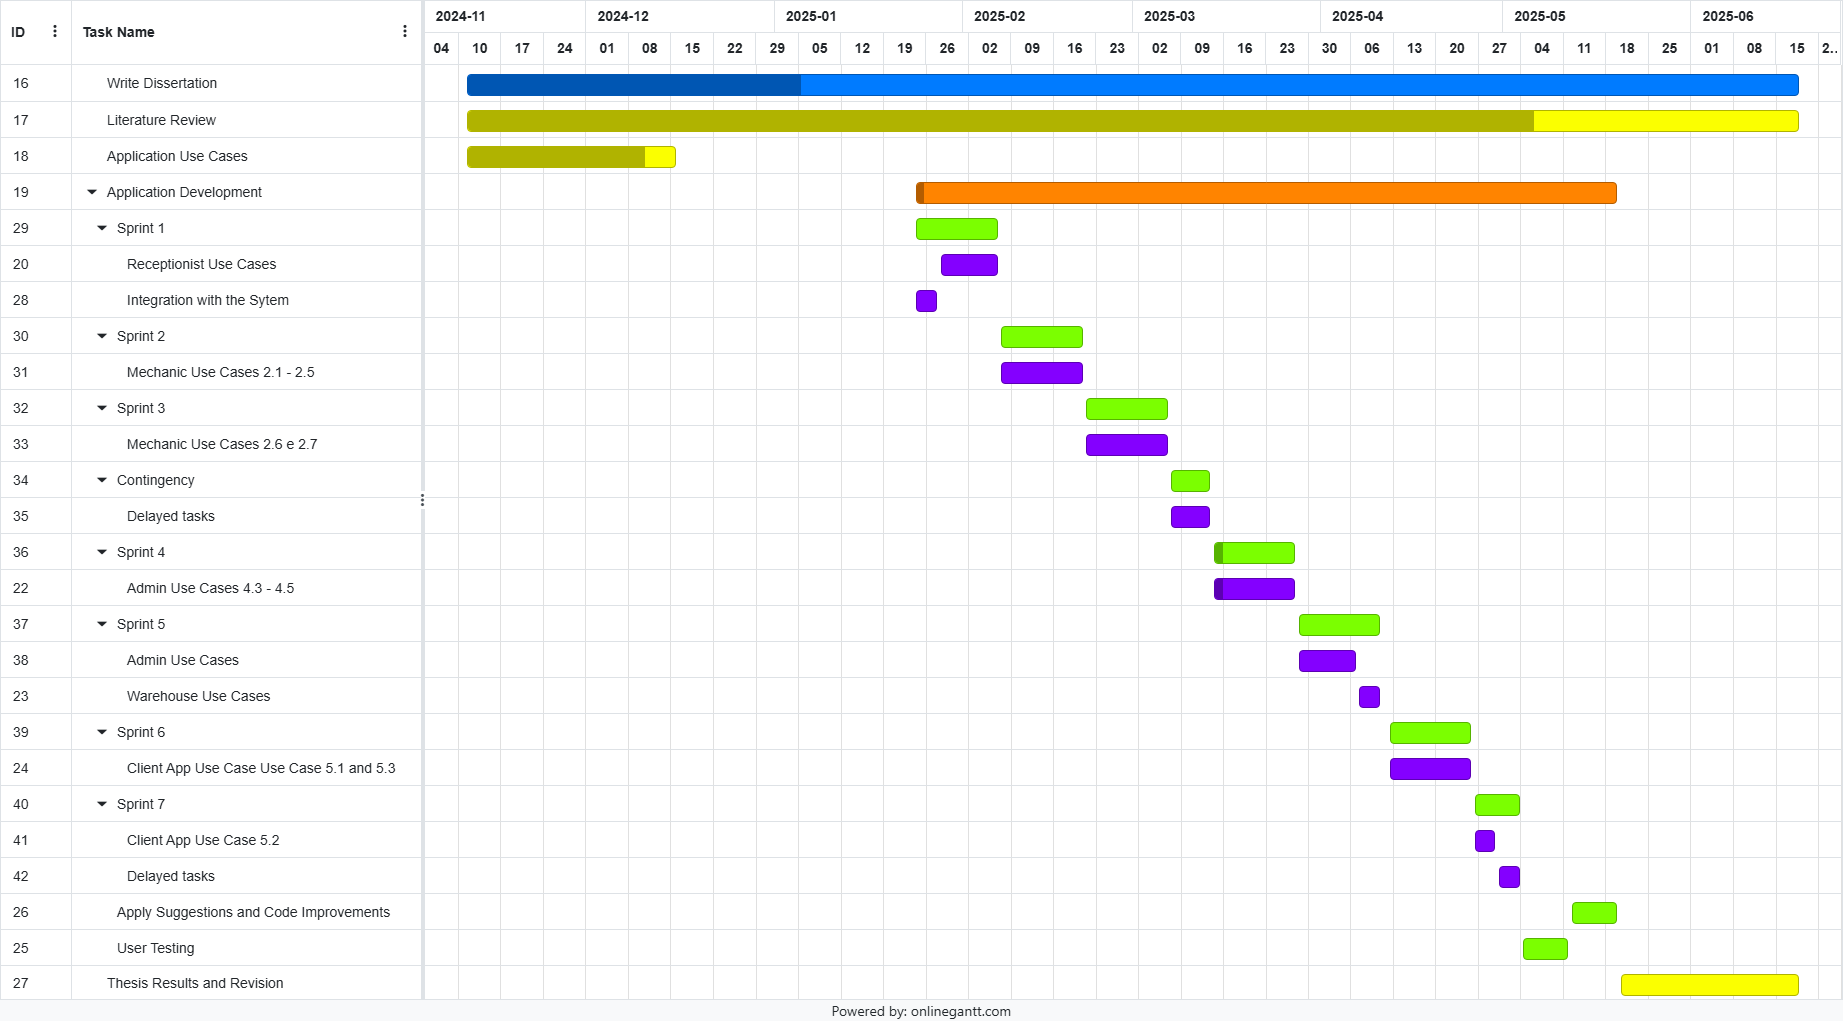
\includegraphics[width=\textwidth]{figs/Gantt}
      \label{fig:figure1}
    \end{figure}
